\documentclass[10pt, pscyr, nonums]{hedlabwork}
\usepackage[russian]{babel}
\usepackage{hedmaths}
\usepackage{graphicx}
\graphicspath{{images/}, {plots/}}

\newgeometry{top=1.5cm, bottom=1.5cm, left=1cm, right=1cm}

\student{Слоква В. И., Ф-469}
\date{30.10.2013}
\labnum{508}
\labname{Лазер}

\begin{document}
  \makeheader

  \emph{Цель работы:} ознакомление с принципом действия гелий-неонового
  оптического квантового генератора (ОКГ) и изучение некоторых характеристик
  лазерного излучения.

  \emph{Используемые при расчетах формулы:}
  \( \phi = \arctg\frac{h}{l}, d\sin\phi = k\lambda,
    \alpha = \arctg\frac{|D_1 - D_2|}{2l}, I_1 = I - I_\varphi \).

  \begin{figure}[h!]
    \center
    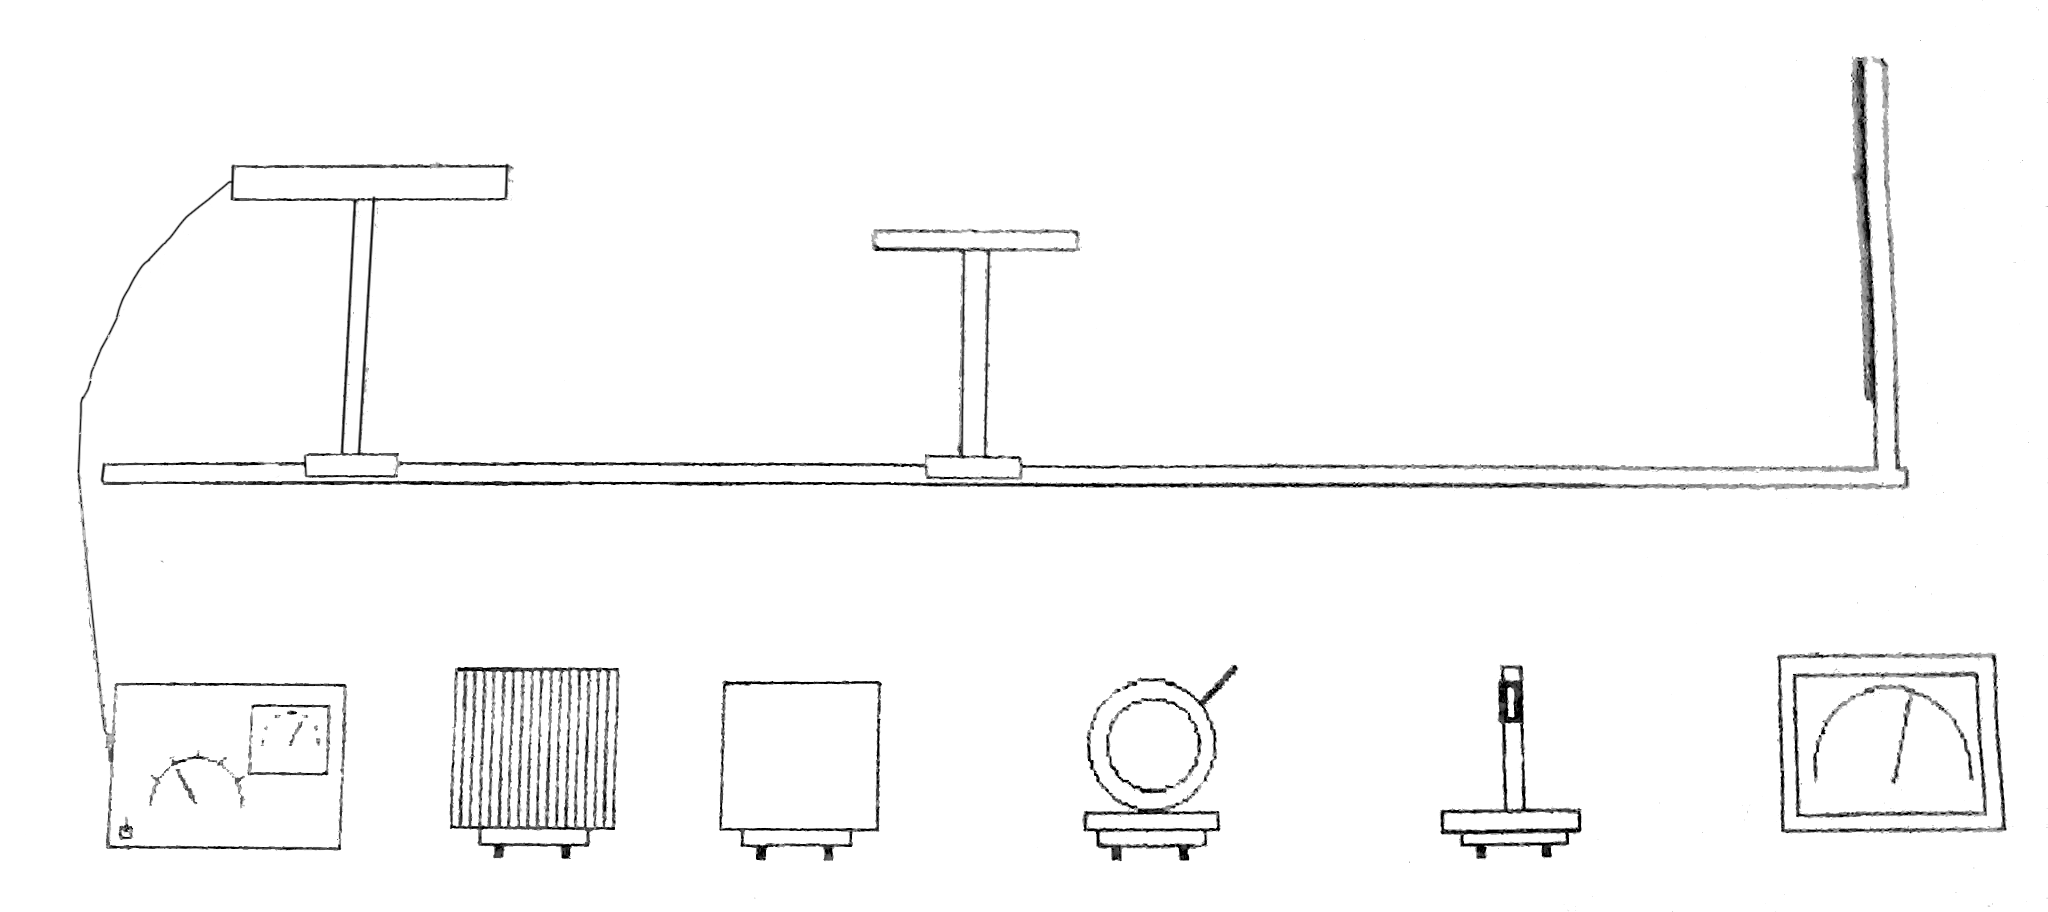
\includegraphics[width=.4\textwidth]{appearance}\\
    \parbox{.4\textwidth}{\caption{Внешний вид установки}}
  \end{figure}
  \vspace*{-2em}

  \begin{table}[h!]
    \center \caption{Определение длины волны излучения лазера}
    \begin{tabular}{|*{8}{C{.08}|}} \hline
      \( d \), мм & \( l \), мм & \( k \) & \( h \), мм &
        \( \phi \), град & \( \sin\phi \) & \( \lambda \), нм &
        \( \midnum{\lambda} \), нм \\ \hline
      \multirow{4}{*}{0,01} & \multirow{2}{*}{900} &
        1 & 60  & 3,81 & 0,067 & \( 665 \pm 13 \)
        & \multirow{4}{*}{\( 665 \pm 13 \)} \\ \cline{3-7}
      &&
        2 & 120 & 7,60 & 0,132 & \( 661 \pm  9 \)
        & \\ \cline{2-7}
      & \multirow{2}{*}{700} &
        1 & 46  & 3,76 & 0,066 & \( 656 \pm 17 \)
        & \\ \cline{3-7}
      &&
        2 & 96  & 7,81 & 0,136 & \( 679 \pm 12 \)
        & \\ \hline
    \end{tabular}
  \end{table}

  \begin{table}[h!]
    \center \caption{Оценка направленности излучения лазера}
    \begin{tabular}{|*{7}{C{.08}|}} \hline
      & \( l \), мм & \( 1 \), мм & \( 2 \), мм & \( 3 \), мм &
        \( \midnum{D} \), мм & \( \alpha \) \\ \hline
      \( D_1 \) & \multirow{2}{*}{800} &
        3 & 3 & 3 & 3 &
        \multirow{2}{*}{\( 4,\!65\cdot 10^{-2} \)} \\ \cline{1-1}\cline{3-6}
      \( D_2 \) &&
        4 & 4 & 5 & 4,3 & \\ \hline
    \end{tabular}
  \end{table}

  \begin{table}[h!]
    \center \caption{Наблюдение и подтверждение линейной поляризации
      излучения лазера}
      \begin{tabular}{|*{2}{*{3}{C{.08}|}|}*{3}{C{.08}|}} \hline
        \( \phi \), град & \( I \), мкА & \( I_1 \), мкА &
          \( \phi \), град & \( I \), мкА & \( I_1 \), мкА &
          \( \phi \), град & \( I \), мкА & \( I_1 \), мкА \\ \hline
        0   & 25 & 21 & 60  & 11 & 7 & 120 & 14 & 10 \\
        5   & 25 & 21 & 65  & 10 & 6 & 125 & 15 & 11 \\
        10  & 24 & 20 & 70  &  8 & 4 & 130 & 16 & 12 \\
        15  & 23 & 19 & 75  &  7 & 3 & 135 & 18 & 14 \\
        20  & 22 & 18 & 80  &  5 & 1 & 140 & 19 & 15 \\
        25  & 21 & 17 & 85  &  4 & 0 & 145 & 20 & 16 \\
        30  & 20 & 16 & 90  &  5 & 1 & 150 & 21 & 17 \\
        35  & 19 & 15 & 95  &  6 & 2 & 155 & 22 & 18 \\
        40  & 17 & 13 & 100 &  7 & 3 & 160 & 22 & 18 \\
        45  & 16 & 12 & 105 &  8 & 4 & 165 & 23 & 19 \\
        50  & 15 & 11 & 110 & 10 & 6 & 170 & 24 & 20 \\
        55  & 13 &  9 & 115 & 12 & 8 & 175 & 24 & 20 \\ \cline{1-6}
        \multicolumn{6}{|c||}{\( I_\varphi = 4 \) мкА \hspace*{4em}} &
          180 & 24 & 20 \\ \hline
        \end{tabular}
  \end{table}
  
  \emph{Подсчет погрешности} определения длины волны проводился по формуле
  \[
    \Delta\lambda = \sqrt{\left( \pder{\lambda}{h}\Delta h \right)^2
    + \left( \pder{\lambda}{l}\Delta l \right)^2},
  \]
  где \( \Delta l = 10 \), \( \Delta h = 1 \), а производные
  \[
    \pder{\lambda}{h} = \frac{d}{k}\cos\left( \arctg\frac{h}{l} \right)\cdot
    \frac{1}{1 + \left( \frac{h}{l} \right)^2}\cdot\frac{1}{l}, \quad
    \pder{\lambda}{l} = \frac{d}{k}\cos\left( \arctg\frac{h}{l} \right)\cdot
    \frac{1}{1 + \left( \frac{h}{l} \right)^2}\cdot\frac{-h}{l^2}.
  \]
  
  \emph{Вывод:} в ходе лабораторной работы были определены некоторые
    характеристики лазерного излучения: угол расхождения очень мал, поляризация
    линейна, длина волны \( \lambda = 665 \pm 15 \)~нм (красный цвет).
\end{document}
